\documentclass[12pt]{article}
\usepackage[margin=48pt]{geometry}
\usepackage{amsthm}
\usepackage{parskip}
\usepackage{graphicx}
\usepackage{enumerate}
\usepackage{subfigure}
\usepackage[usenames]{color}


\begin{document}

\thispagestyle{empty}
\hrule
\vspace{1em}
\begin{center}
{\Huge \LaTeX{} Practical Template} \\
\vspace{2em}
Author Name
\end{center}
\vspace{2em}
\hrule

\vspace{4em}

\begin{center}
{\Large \bf Summary}
\end{center}

Put the scientific summary here.

\vspace{4em}

\tableofcontents

\vfill

\hrule

\newpage
\setcounter{page}{1}
\section{Including Figures from R}

First create a figure in R using the \texttt{pdf} function.

\begin{verbatim}
  pdf("figure.pdf", width = 6, height = 4, bg = "white")
  plot(NA, NA, xlim = c(0, 20), ylim = c(1.7, 5), xlab = "",
       ylab = "", type = "n", axes = F)

  x <- seq(1, 19, length = 1901)
  y <- 0.015 * (x - 12.5)^2 + 3
  lines(x, y)

  for(i in 0:6) {
    x <- 3*i+1
    segments(x, 2.6, x, 2.75)
    text(x, 2.4, letters[1])
    text(x + 0.3, 2.35, i+1, cex = 0.7)
  }
  segments(1, 2.675, 19, 2.675)

  segments(10, 2.05, 10, 2.15)
  segments(16, 2.05, 16, 2.15)
  segments(13, 2.05, 13, 2.25)
  segments(10, 2.1, 16, 2.1)

  for(x in c(11, 12, 14, 15))
    segments(x, 2.05, x, 2.15)

  for(i in 0:6) {
    x <- i + 10
    text(x, 1.85, letters[2])
    text(x + 0.3, 1.8, i+1, cex = 0.7)
  }

  box()
  dev.off()
\end{verbatim}




\newpage
\pagecolor{yellow}
\begin{figure}[h]
  \centering
  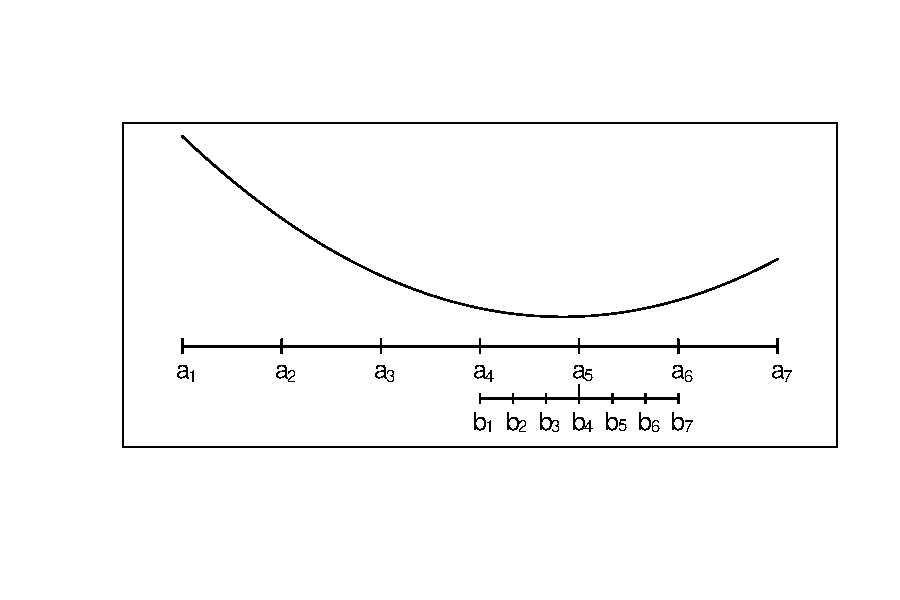
\includegraphics{figure.pdf} 
  \caption{Put caption here.\label{fig:minalg}}
\end{figure}

There is a lot of white space around the figure and it is not centered.  This happens because R leaves space for axis labels and for a title at the top of the figure.  You can trim off the white space using the \texttt{trim} and \texttt{clip} arguments for \texttt{includegraphics}.

\begin{verbatim}
  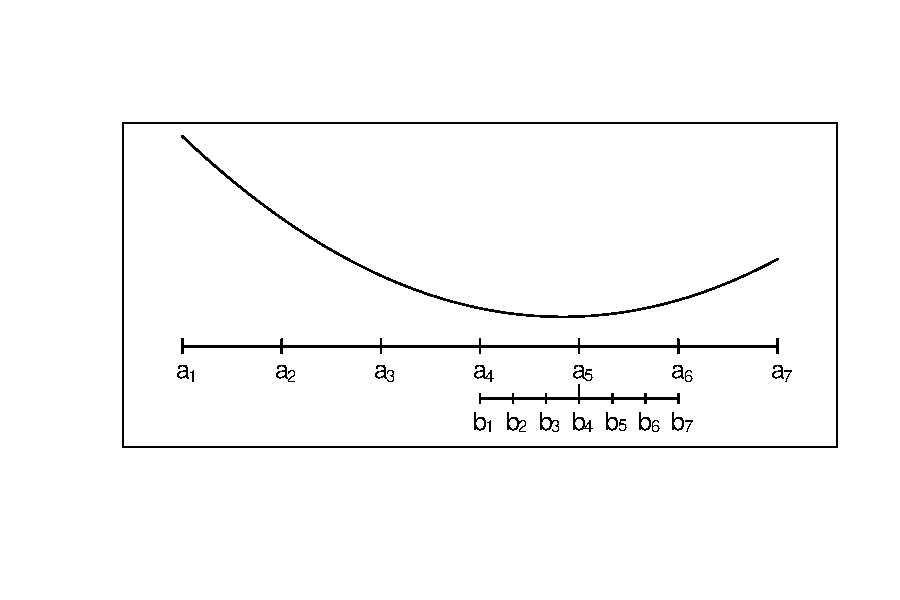
\includegraphics[trim=10px 20px 30px 40px, clip]{figure.pdf} 
\end{verbatim}

The order of those $4$ lengths is left, bottom, right, top.  After some guessing and checking I found 

\begin{verbatim}
  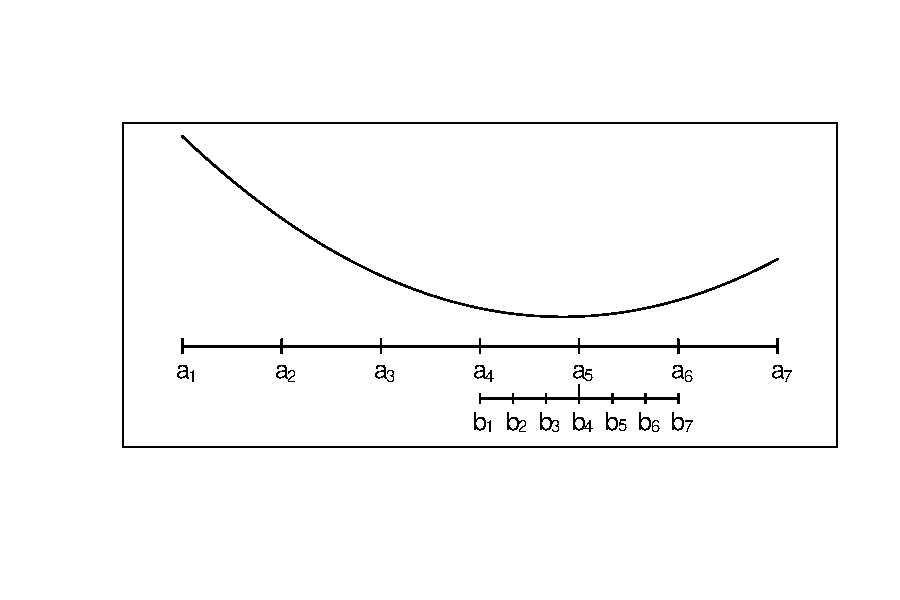
\includegraphics[trim=50px 65px 22px 50px, clip]{figure.pdf}
\end{verbatim}

gives a good result.

Note: please do not actually use yellow pages in your report.

\newpage
Figure \ref{fig:minalg1} looks much better.

\begin{figure}[h]
  \centering
  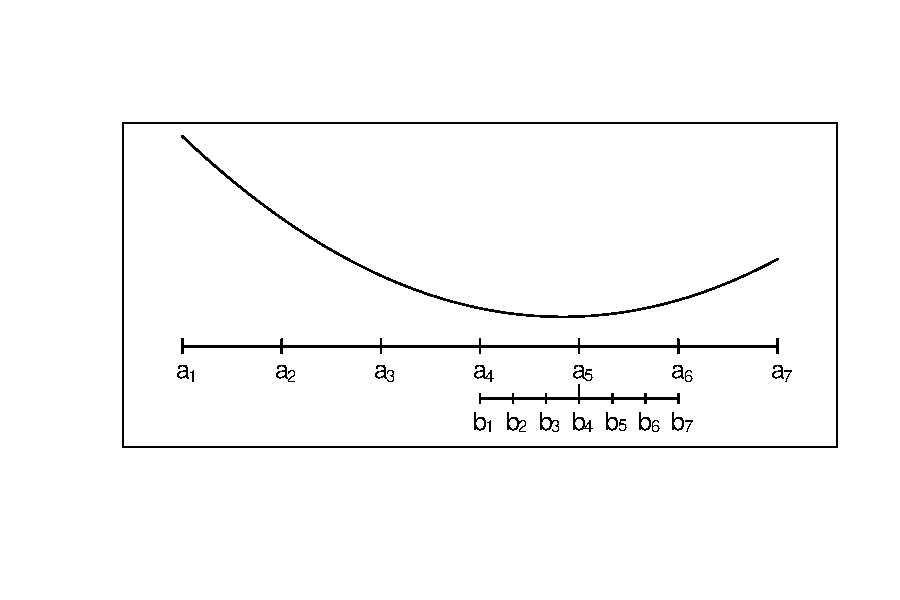
\includegraphics[trim=50px 65px 22px 50px, clip]{figure.pdf} 
  \caption{Same figure with less wasted space.\label{fig:minalg1}}
\end{figure}


\newpage
\pagecolor{white}

\section{Using Subfigures}

If you want more than one plot in the same figure then use subfigure.  You need to include the subfigure package by putting \texttt{\char`\\usepackage\{subfigure\}} in the header of your .tex file.  Here are the four plots generated by plot.lm.  You should experiment with using \texttt{\char`\\ref} to use cross references for your subfigures.  For instance, I like figure \ref{subfig:qq}.

Note: you should use the \texttt{xlab}, \texttt{ylab}, and \texttt{main} arguments when making your plots rather than accept R's default labels.

\begin{figure}[h]
\centering
\subfigure[Residuals vs. Fitted Values\label{subfig:rf}]{
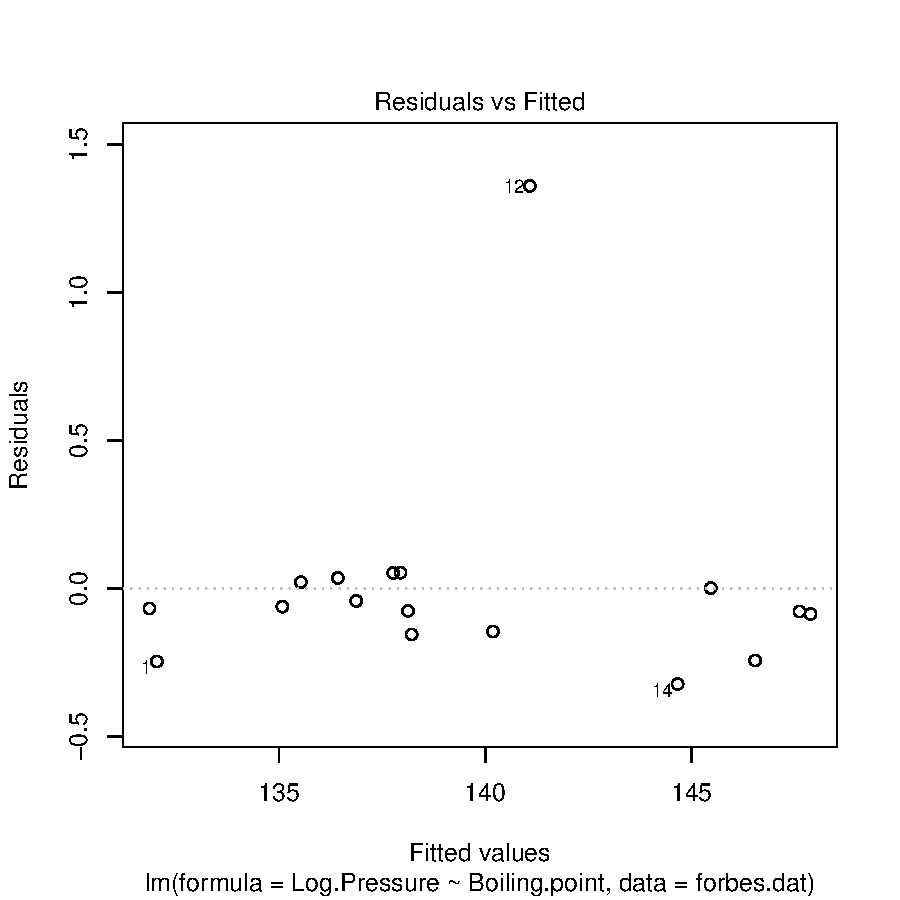
\includegraphics[width=3in]{rf.pdf}
}
\subfigure[Normal QQ Plot of the Residuals\label{subfig:qq}]{
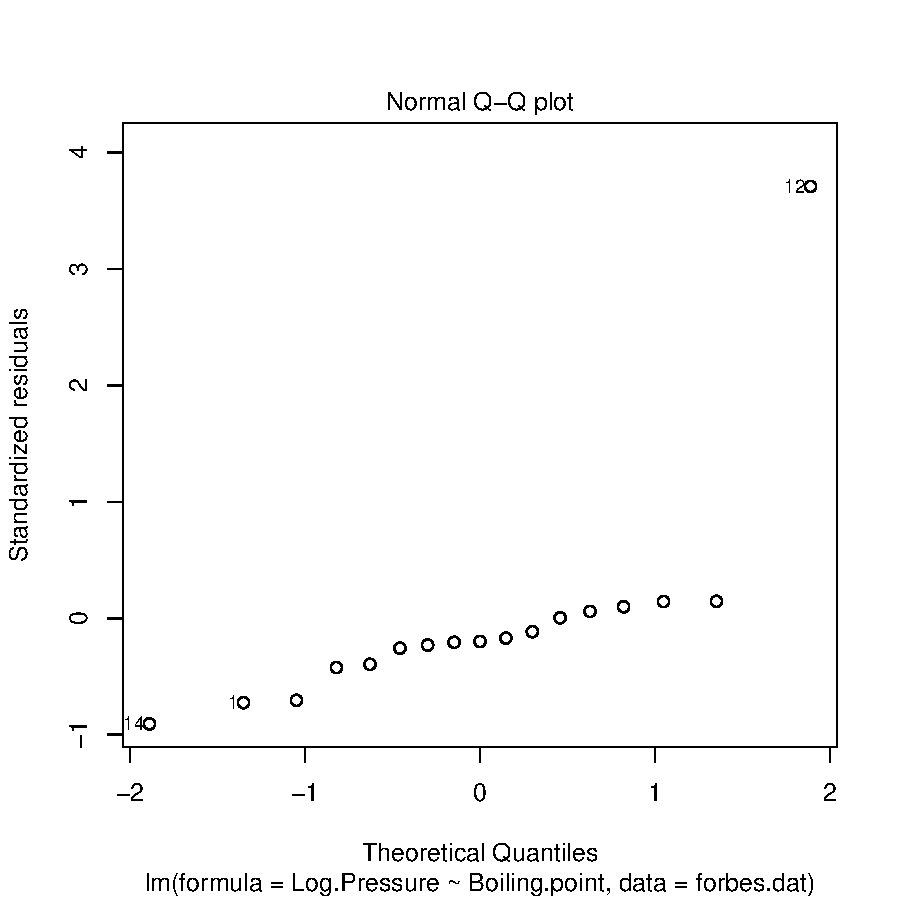
\includegraphics[width=3in]{qq.pdf}
}
\subfigure[Scale-Location Plot\label{subfig:sl}]{
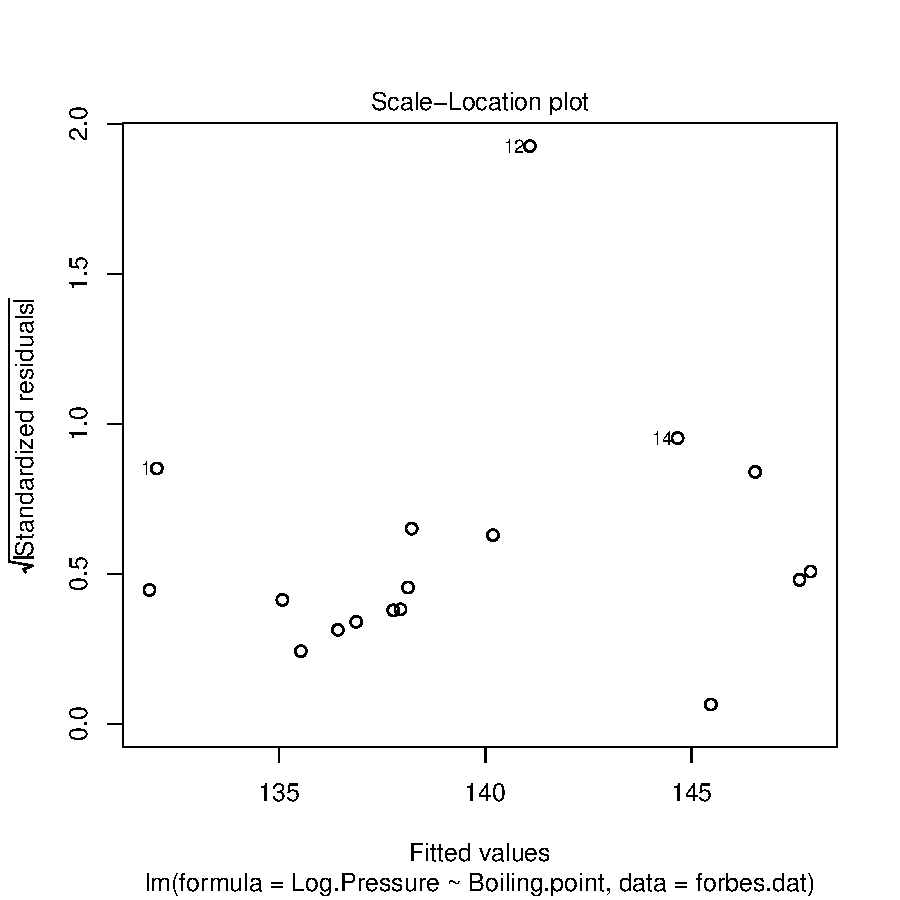
\includegraphics[width=3in]{sl.pdf}

}
\subfigure[Cook's Distance\label{subfig:cd}]{
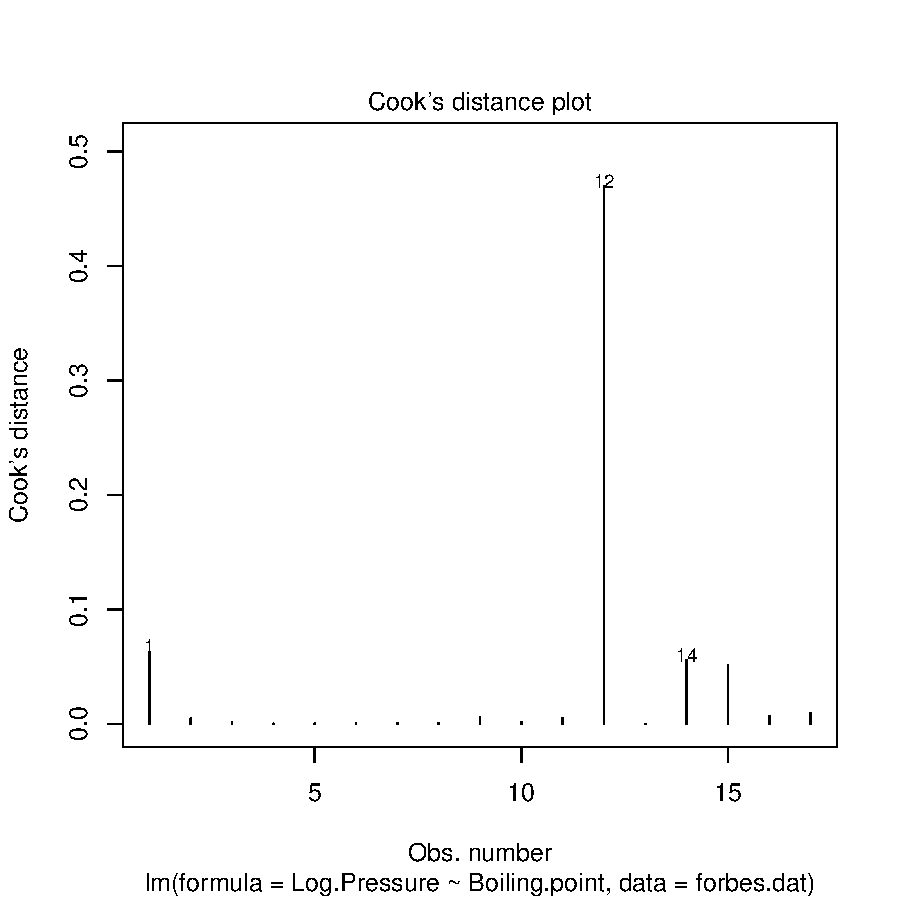
\includegraphics[width=3in]{cd.pdf}
}
\caption{The plot method for R linear model objects.\label{fig:lmplots}}
\end{figure}



\newpage
\section{Including Tables}

\begin{table}[h]
\begin{center}
\caption{Forbes' data on the air pressure in the Alps and the boiling point of water.\label{tab:forbes}}
\vspace{1em}
\begin{tabular}{ccc} \hline
Observation & Boiling & $100 \times$ \\
Number & Point ($^{\circ}$F) & Log(Pressure) \\ \hline
1 & 194.5 & 131.79 \\
2 & 194.3 & 131.79 \\
3 & 197.9 & 135.02 \\
4 & 198.4 & 135.55 \\
5 & 199.4 & 136.46 \\
6 & 199.9 & 136.83 \\
7 & 200.9 & 137.82 \\
8 & 201.1 & 138 \\
9 & 201.4 & 138.06 \\
10 & 201.3 & 138.05 \\
11 & 203.6 & 140.04 \\
12 & 204.6 & 142.44 \\
13 & 209.5 & 145.47 \\
14 & 208.6 & 144.34 \\
15 & 210.7 & 146.3 \\
16 & 211.9 & 147.54 \\
17 & 212.2 & 147.8 \\ \hline
\end{tabular}
\end{center}
\end{table}

\newpage
\section{Citations}
I am going to cite Atkinson \cite{atkinson85}, Cook \cite{cook77} and Woodbury \cite{woodbury50} just so that they show up in the references.


\newpage
\appendix
\section{This is an appendix}

Appendices are just like sections except that they come after the \texttt{\char`\\appendix} tag in your .tex file.

\newpage
\bibliography{references}
\bibliographystyle{plain}

% Add the References to the table of contents.
\addcontentsline{toc}{section}{References}

\end{document}
